\documentclass[12pt, oneside]{article}
\usepackage[letterpaper, margin=1in, headsep=0.5in]{geometry}
\usepackage[english]{babel}
\usepackage[utf8]{inputenc}
\usepackage{amsmath}
\usepackage{amsfonts}
\usepackage{amssymb}
\usepackage{tikz}
\usetikzlibrary{quotes, angles}
\usepackage{graphicx}
%\usepackage{pgfplots}
%\pgfplotsset{width=10cm,compat=1.9}
%\usepgfplotslibrary{statistics}
%\usepackage{pgfplotstable}
%\usepackage{tkz-fct}
%\usepackage{venndiagram}

\usepackage{fancyhdr}
\pagestyle{fancy}
\fancyhf{}
\rhead{\thepage \\Name: \hspace{1.5in}.\\}
\lhead{BECA / Dr. Huson / 10th Grade Geometry\\* Unit 4: Parallels and transversals \\ 28 October 2019}

\renewcommand{\headrulewidth}{0pt}

\begin{document}
\subsubsection*{Classwork: Constructions using perpendicular bisection}
Use only a compass and straightedge for these classical constructions.
  \begin{enumerate}

  \item Construct a perpendicular bisector the given line segment $\overline{AB}$. Label the midpoint of $\overline{AB}$ as $M$.  [Leave all construction marks.]\\
    \vspace{1cm}
    \begin{center}
    \begin{tikzpicture}
      \draw [-, thick] (0,3)--(3,0);
      \draw [fill] (0,3) circle [radius=0.05] node[above left]{$A$};
      %\node at (8.5,-0.4){$l$};
      \draw [fill] (3,0) circle [radius=0.05] node[below right]{$B$};
    \end{tikzpicture}
    \end{center}
    \vspace{3cm}

  \item Construct a perpendicular to $\overline{AB}$ though $C$.\\
  Hint: Start with a circle centered on $C$.
    %\hspace{1cm} Given the line  $l$ and point $P$.
    \vspace{4cm}
    \begin{center}
    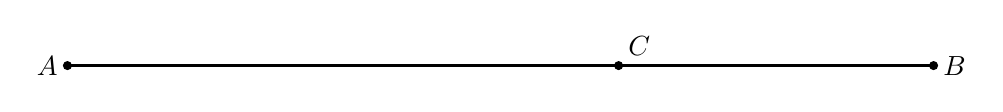
\begin{tikzpicture}
      \draw [-, thick] (0,0)--(11,0);
      \draw [fill] (0,0) circle [radius=0.05] node[left]{$A$};
      \draw [fill] (11,0) circle [radius=0.05] node[right]{$B$};
      \draw [fill] (7,0) circle [radius=0.05] node[above right]{$C$};
    \end{tikzpicture}
  \end{center} %\vspace{3cm}

\newpage
\subsubsection*{Construct a triangle's circumcenter}

  \item Construct a perpendicular bisector of each of the legs of the triangle. Show their intersection, the circumcenter.\\[0.2cm]
  Hint: Circles should be centered at the triangle vertices, but should only be sufficiently large to intersect the other circles.
      %\hspace{1cm} Given the line  $l$ and point $P$.
      \vspace{3cm}
      \begin{center}
      \begin{tikzpicture}
        \draw [<->, thick] (0,0)--(9,0)--(7,11)--cycle;
        %\draw [fill] (2,3) circle [radius=0.05] node[right]{$P$};
        %\node at (8.5,-0.4){$l$};
        %\draw [fill] (6,0) circle [radius=0.05] node[below]{$Q$};
      \end{tikzpicture}
      \end{center}

  \newpage
  \subsubsection*{Construct a triangle's centroid}

    \item Bisect each leg of the triangle using only a compass and straightedge. Mark each midpoint, and draw a line (a \emph{median}) connecting it to the opposite vertex. Show the medians' intersection, the centroid.\\[0.2cm]
    Hint: Circles should be centered at the triangle vertices, but should only be sufficiently large to intersect the other circles.
        %\hspace{1cm} Given the line  $l$ and point $P$.
        \vspace{3cm}
        \begin{center}
        \begin{tikzpicture}
          \draw [<->, thick] (0,0)--(9,0)--(7,11)--cycle;
          %\draw [fill] (2,3) circle [radius=0.05] node[right]{$P$};
          %\node at (8.5,-0.4){$l$};
          %\draw [fill] (6,0) circle [radius=0.05] node[below]{$Q$};
        \end{tikzpicture}
        \end{center}

\end{enumerate}
\end{document}
